\documentclass{beamer}

\mode<presentation> {

% The Beamer class comes with a number of default slide themes
% which change the colors and layouts of slides. Below this is a list
% of all the themes, uncomment each in turn to see what they look like.

%\usetheme{default}
%\usetheme{AnnArbor}
%\usetheme{Antibes}
%\usetheme{Bergen}
%\usetheme{Berkeley}
%\usetheme{Berlin}
%\usetheme{Boadilla}
%\usetheme{CambridgeUS}
%\usetheme{Copenhagen}
%\usetheme{Darmstadt}
%\usetheme{Dresden}
\usetheme{Frankfurt}
%\usetheme{Goettingen}
%\usetheme{Hannover}
%\usetheme{Ilmenau}
%\usetheme{JuanLesPins}
%\usetheme{Luebeck}
%\usetheme{Madrid}
%\usetheme{Malmoe}
%\usetheme{Marburg}
%\usetheme{Montpellier}
%\usetheme{PaloAlto}
%\usetheme{Pittsburgh}
%\usetheme{Rochester}
%\usetheme{Singapore}
%\usetheme{Szeged}
%\usetheme{Warsaw}

% As well as themes, the Beamer class has a number of color themes
% for any slide theme. Uncomment each of these in turn to see how it
% changes the colors of your current slide theme.

%\usecolortheme{albatross}
%\usecolortheme{beaver}
%\usecolortheme{beetle}
\usecolortheme{crane}
%\usecolortheme{dolphin}
%\usecolortheme{dove}
%\usecolortheme{fly}
%\usecolortheme{lily}
%\usecolortheme{orchid}
%\usecolortheme{rose}
%\usecolortheme{seagull}
%\usecolortheme{seahorse}
%\usecolortheme{whale}
%\usecolortheme{wolverine}

%\setbeamertemplate{footline} % To remove the footer line in all slides uncomment this line
%\setbeamertemplate{footline}[page number] % To replace the footer line in all slides with a simple slide count uncomment this line

%\setbeamertemplate{navigation symbols}{} % To remove the navigation symbols from the bottom of all slides uncomment this line
}

\usepackage{extpfeil}
\usepackage{extarrows} %Allows long equation signs
\usepackage{graphicx} % Allows including images
\usepackage{booktabs} % Allows the use of \toprule, \midrule and \bottomrule in tables
\usepackage{physics}
\usepackage{tikz}
\usepackage{cite}
%花体字母
\usepackage{amsthm,amsmath,amssymb}
\usepackage{mathrsfs}
\usepackage{dutchcal}
\usepackage{circuitikz}
\usepackage{multirow}

%----------------------------------------------------------------------------------------
%	TITLE PAGE
%----------------------------------------------------------------------------------------

\title[VP260 RC]{Final Review} % The short title appears at the bottom of every slide, the full title is only on the title page

\author{VP260 TA Group} % Your name
\institute[UM-SJTU JI] % Your institution as it will appear on the bottom of every slide, may be shorthand to save space
{
    University of Michigan - Shanghai Jiao Tong University Joint Institute\\% Your institution for the title page
\medskip
}
\date{\today} % Date, can be changed to a custom date

\AtBeginSection[]
{
  \begin{frame}
    \frametitle{Table of Contents}
    \tableofcontents[currentsection]
  \end{frame}
}

\begin{document}

\begin{frame}
    \titlepage % Print the title page as the first slide
\end{frame}

\begin{frame}{Outline}
    \tableofcontents
\end{frame}

%----------------------------------------------------------------------------------------
%	 SECTION 1
%----------------------------------------------------------------------------------------
\section{Fundamental Concepts}

\subsection{Maxwell's Equation} % Section title slide, unnumbered

\begin{frame}{Faraday’s Law and Lenz' Law}
    A changing magnetic field induces an electric field.

    \begin{block}{Faraday's law}
        \begin{equation}
            \oint \va{E} \vdot \dd{\va{l}} = -\oint \pdv{\va{B}}{t} \dd{\va{a}}
        \end{equation}

        \begin{equation}
            \curl{\va{E}} = -\pdv{\va{B}}{t}
        \end{equation}
    \end{block}

    \begin{block}{Lenz' law}
        The negative sign means that nature abhors a change in flux.
    \end{block}
\end{frame}

\begin{frame}{Displacement Current}
    A changing electric field induces a magnetic field.

    \begin{columns}
        \begin{column}{0.5\textwidth}
            \begin{figure}[htbp]
                \centering
                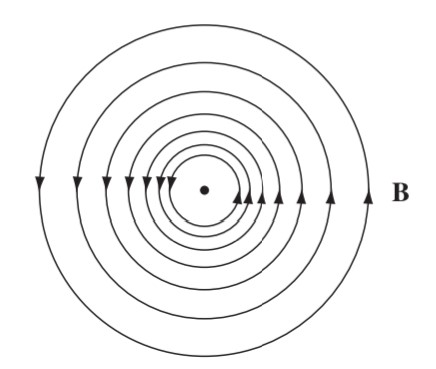
\includegraphics[width=\textwidth]{Images/amp.jpg}
            \end{figure}
        \end{column}
        \begin{column}{0.5\textwidth}
            \begin{block}{Displacement current}
                \begin{equation}
                    \va{J}_d = \epsilon_0 \pdv{\va{E}}{t}
                \end{equation}
            \end{block}
        \end{column}
    \end{columns}
\end{frame}

\begin{frame}{Maxwell's Equation}
    \begin{table}[htbp]
        \centering
        \begin{tabular}{ll}
            \toprule
            Integral Form                                                                         & Differential Form                                              \\
            \midrule
            $\oint \va{E}\vdot\dd{\va{a}}=\frac{Q_{\text{enc}}}{\epsilon_0}$                      & $\div{\va{E}} = \frac{\rho}{\epsilon_0}$                       \\ \addlinespace
            $\oint \va{E}\vdot\dd{\va{l}}= -\dv{\Phi_B}{t}$                                       & $\curl{\va{E}}=-\pdv{\va{B}}{t}$                               \\ \addlinespace
            $\oint \va{B}\vdot\dd{\va{a}}=0$                                                      & $\div{\va{B}} = 0$                                             \\ \addlinespace
            $\oint \va{B}\vdot\dd{\va{l}}=\mu_0 I_{\text{enc}} + \mu_0 \epsilon_0 \dv{\Phi_E}{t}$ & $\curl{\va{B}}=\mu_0 \va{J}+ \mu_0 \epsilon_0 \pdv{\va{E}}{t}$ \\
            \bottomrule
        \end{tabular}
    \end{table}
\end{frame}

\subsection{Magnetic Vector Potential}

\begin{frame}{Scalar and Vector Potentials}
    \begin{block}{Vector Potential}
        \begin{equation}
            \va{B} = \curl \va{A}
        \end{equation}
        \begin{equation}
            \va{E} = -\grad V - \pdv{\va{A}}{t}
        \end{equation}
    \end{block}

    \begin{block}{Gauge Transform}
        \begin{equation}
            \va{A}'=\va{A}+\nabla \lambda
        \end{equation}
        \begin{equation}
            V'=V-\frac{\partial \lambda}{\partial t}
        \end{equation}
    \end{block}
\end{frame}

\begin{frame}{Gauge}
    \begin{block}{Coulomb Gauge}
        \begin{equation*}
            \div\va{A} = 0
        \end{equation*}
    \end{block}

    \begin{block}{Lorenz Gauge}
        \begin{equation*}
            \div \va{A} = -\mu_0\epsilon_0\pdv{V}{t}
        \end{equation*}
    \end{block}

    \begin{block}{Landau Gauge}
        For uniform magnetic field $\va{B} = B \vu{z}$,
        \begin{equation*}
            \va{A} = By \vu{x}
        \end{equation*}
    \end{block}
\end{frame}

\subsection{Inductance}

\begin{frame}{Inductance (unit: H)}
    \begin{block}{Mutual Inductance}
        \begin{equation}
            M_{21}=\frac{\mu_{0}}{4 \pi} \oint \oint \frac{d \mathbf{l}_{1} \cdot d \mathbf{l}_{2}}{r}
        \end{equation}
        \begin{equation}
            M_{21} = M_{12}
        \end{equation}
        \begin{equation}
            \Phi_2 = M I_1
        \end{equation}
    \end{block}

    \begin{block}{Self Inductance}
        \begin{equation}
            \Phi = L I
        \end{equation}
        \begin{equation}
            \varepsilon = - L \dv*{I}{t}
        \end{equation}

        Pay attention to the direction (potential drop through inductor).
    \end{block}

    \begin{itemize}
        \item Inductor: $W_L = \frac{1}{2} L I^2$
        \item Magnetic field energy density: $u = \frac{B^2}{2 \mu_r\mu_0}$
    \end{itemize}
\end{frame}

\subsection{RLC \& AC Circuits}

\begin{frame}{RL, LC, RLC Circuits}
    \begin{table}[htbp]
        \centering
        \begin{tabular}{l c l}
            \toprule
            RC                   & $i(t)=\epsilon/R(1-exp(-t/\tau))$                                                                 & $\tau=RC$               \\ \addlinespace[1em]
            RL                   & $i(t)=\epsilon/R(1-exp(-t/\tau))$                                                                 & $\tau=L/R$              \\ \addlinespace[1em]
            LC                   & $q(t) = A\sin(\omega_0 t) + B\cos(\omega_0 t)$                                                    & $\omega_0 = 1\sqrt{LC}$ \\ \addlinespace[1em]
            \multirow{3}{*}{RLC} & \multirow{3}{*}{$\frac{d^{2} I(t)}{d t^{2}}+\frac{R}{L} \frac{d I(t)}{d t}+\frac{1}{L C} I(t)=0$} & Underdamped             \\
                                 &                                                                                                   & Critical damping        \\
                                 &                                                                                                   & Overdamped              \\
            \bottomrule
        \end{tabular}
    \end{table}
\end{frame}


\begin{frame}{AC Circuit}
    \begin{block}{AC current}
        \begin{equation}
            i(t) = I_0 \cos(\omega t + \phi)
        \end{equation}
        \begin{equation}
            i(t) = \Re{I_0 e^{\phi j} e^{j\omega t}}
        \end{equation}
    \end{block}
    \begin{itemize}
        \item Rectified average current: $I_{rav} = \frac{1}{T}\int_{t_1}^{t_1+T}\abs{i(t)}\dd t = \frac{2}{\pi}I$
        \item Root-mean-square current: $I_{rms} = \sqrt{\frac{1}{T}\int_{t_1}^{t_1+T}i^2(t)\dd t} = \frac{I}{\sqrt{2}}$
    \end{itemize}
\end{frame}

\begin{frame}{Elements in AC}
    \begin{table}[htbp]
        \centering
        \begin{tabular}{l c c}
            \toprule
            Elements & Impedance        & Phase    \\
            \midrule
            R        & $R$              & 0        \\
            L        & $j\omega L $     & $\pi/2$  \\
            C        & $1/(j \omega C)$ & $-\pi/2$ \\
            \bottomrule
        \end{tabular}
    \end{table}

    \begin{block}{Resonance}
        \begin{equation}
            \abs{Z} = \sqrt{R^2+(\omega L - \frac{1}{\omega C})^2 }
        \end{equation}
        Resonance happens when $\omega_0 = \frac{1}{LC}$
    \end{block}

    \begin{block}{ Power}
        \begin{equation}
            \overline{P} = V_{rms} I_{rms}
        \end{equation}
    \end{block}
\end{frame}

\subsection{Electromagnetic Waves}

\begin{frame}{Classical Wave Equation}
    \begin{block}{Classical wave equation}
        \begin{equation}
            \pdv[2]{f}{x} = \frac{1}{v^2} \pdv[2]{f}{t}
        \end{equation}
    \end{block}
    \vfill
    \begin{itemize}
        \item $f$ is displacement, $v$ is speed of propagation;
        \item Example: sound, wave on a string;
        \item Solution: $f(x, t) = g(x - vt) + h(x + vt)$.
    \end{itemize}
\end{frame}

\begin{frame}{Sinusoidal Waves}
    \begin{block}{Sinusoidal wave}
        \begin{equation}
            f(x, t) = A \cos(k (x - vt) + \varphi)
        \end{equation}
    \end{block}

    \begin{block}{Complex wave function}
        \begin{equation}
            \tilde{f}(x, t) = \tilde{A} e^{i(kx-\omega t)}
        \end{equation}
    \end{block}

    \begin{table}[htbp]
        \centering
        %\caption{name}
        \begin{tabular}{ll}
            $A$                        & amplitude                                 \\
            $k$                        & wave number                               \\
            $k(x-vt)+\varphi$          & phase                                     \\
            $\varphi$                  & phase constant ($0 \leq \varphi < 2 \pi$) \\
            $\lambda = \frac{k}{2\pi}$ & wave length                               \\
            $T = \frac{2\pi}{kv}$      & period                                    \\
            $\nu = \frac{1}{T}$        & frequency                                 \\
            $\omega = 2\pi \nu$        & angular frequency                         \\
        \end{tabular}
    \end{table}

\end{frame}


\begin{frame}{Electromagnetic Waves in Vacuum}
    \begin{block}{Electromagnetic waves in vacuum}
        \begin{equation}
            \va{E}(z, t) = E_0 \cos(kz - \omega t + \varphi) \vu{x},
        \end{equation}
        \begin{equation}
            \va{B}(z, t) = \frac{1}{c}E_0 \cos(kz - \omega t + \varphi) \vu{y}.
        \end{equation}
    \end{block}
    \begin{itemize}
        \item Transverse wave;
        \item Two field are in phase and perpendicular;
        \item The direction of polarization is the same as $\va{E}$.
        \item $\tilde{\vb{B}}_0 = \frac{k}{\omega} \left(\vu{z} \times \tilde{\vb{E}}_0 \right) = \frac{1}{c} \left(\vu{z} \times \tilde{\vb{E}}_0 \right)$
    \end{itemize}

    \begin{figure}[htbp]
        \centering
        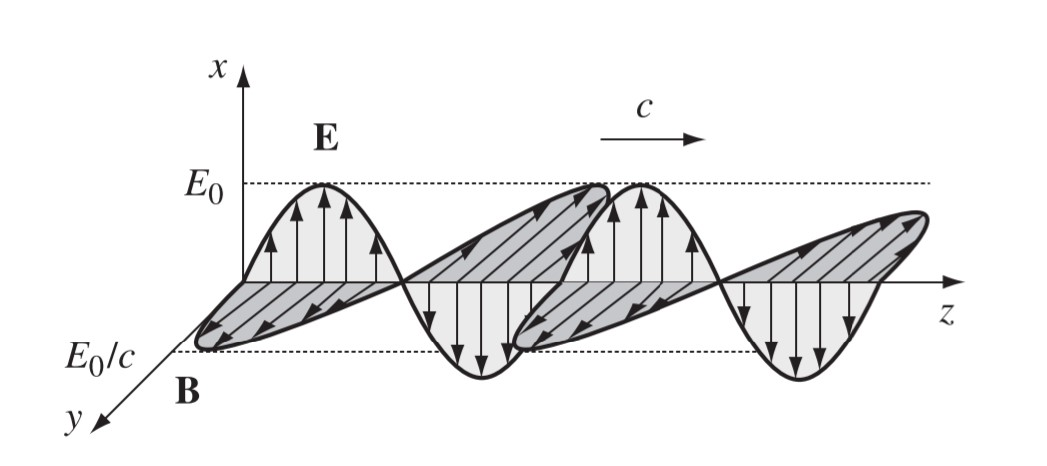
\includegraphics[width=0.5\textwidth]{Images/emwave.jpg}
    \end{figure}
\end{frame}

\begin{frame}{Poynting Vector}
    We define the energy flux (energy per unit area, per unit time) as Poynting vector,

    \begin{block}{Poynting Vector}
        \begin{equation}
            \va{S} = \frac{1}{\mu_0} (\va{E} \times \va{B})
        \end{equation}
    \end{block}

    For the sinusoidal waves, $\va{S} = cu \vu{z}$ where $u = \epsilon_0 E^2$ is energy density.
\end{frame}

\begin{frame}{Standing e-m Wave}
    \begin{beamerboxesrounded}[shadow=true]{Standing Wave Formula}
        Reflected by a perfect conductor:
        \begin{equation}
            \va{E}(z, t) = -2E_0 \sin(kz) \sin(\omega t) \vu{x}
        \end{equation}
        \begin{equation}
            \va{B}(z, t) = -2B_0 \cos(kz) \cos(\omega t) \vu{y}
        \end{equation}
    \end{beamerboxesrounded}
    \vspace{.5em}
    \begin{itemize}
        \item Reflection: direction of $\va{S}$, $\va{E}$ changes; direction of $\va{B}$ does not change.
        \item Node of electric field: $z_n = n \lambda/2$
        \item Node of magnetic field: $z_n = (2n+1)\lambda/4$
    \end{itemize}
\end{frame}



\begin{frame}{Momentum Transport}
    Momentum density: 
    \begin{equation}
        \textbf{$\Pi$} = \frac{1}{c^2}\va{S}
    \end{equation}

    Average momentum density ($\overline{\text{power}}$/area):
    \begin{equation}
        \begin{split}
            \langle u\rangle&=\frac{1}{2} \varepsilon_{0} E_{0}^{2} \\
            \langle \va{s} \rangle &= \frac{1}{2}c\epsilon_0E^2_0 \vu{n} \\ 
            \langle \textbf{$\Pi$} \rangle&= \frac{1}{2c}\epsilon_0 E^2_0 \vu{n}
        \end{split}
    \end{equation}

    \begin{beamerboxesrounded}[shadow=true]{Intensity}
        \begin{equation}
            \text{I} = \abs{\langle \va{s} \rangle} = \frac{1}{2} c \epsilon_0 E^2_0
        \end{equation}        
    \end{beamerboxesrounded}
    \vspace{.5em}

\end{frame}


\subsection{Optics}

\begin{frame}{Reflection and Refraction}
    \begin{columns}
        \begin{column}{.3\linewidth}
            \begin{figure}[htbp]
                \centering
                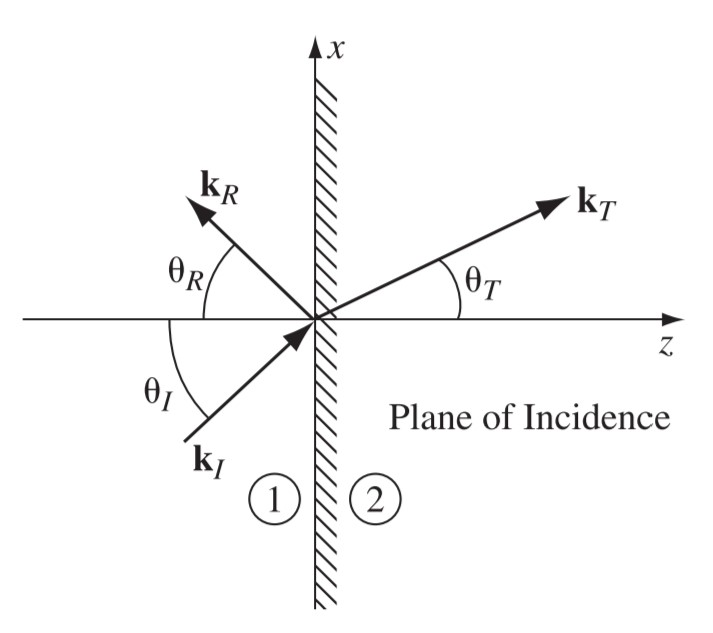
\includegraphics[width=\textwidth]{Images/re.jpg}
            \end{figure}
        \end{column}
        \begin{column}{.7\linewidth}
            \begin{block}{Law of reflection}
                \begin{equation}
                    \theta_I = \theta_R
                \end{equation}
            \end{block}

            \begin{block}{Law of refraction (Snell's law)}
                \begin{equation}
                    \frac{\sin \theta_T}{\sin \theta_I} = \frac{n_1}{n_2}
                \end{equation}
            \end{block}
            \begin{itemize}
                \item $n_i = v_i / c$ is called refractive index.
                \item When $\theta_I > \theta_{cr}$, where $\sin \theta_{cr} = n_2 / n_1$, there is a total internal reflection.
            \end{itemize}
        \end{column}
    \end{columns}
\end{frame}

\begin{frame}{Huygens' Principle}
    \begin{block}{Huygens' principle}
        Every point of the wavefront may be considered as a source of secondary wavelets that propagate out in all directions with speed equal to speed of propagation of the wave.
    \end{block}

    \begin{figure}[htbp]
        \centering
        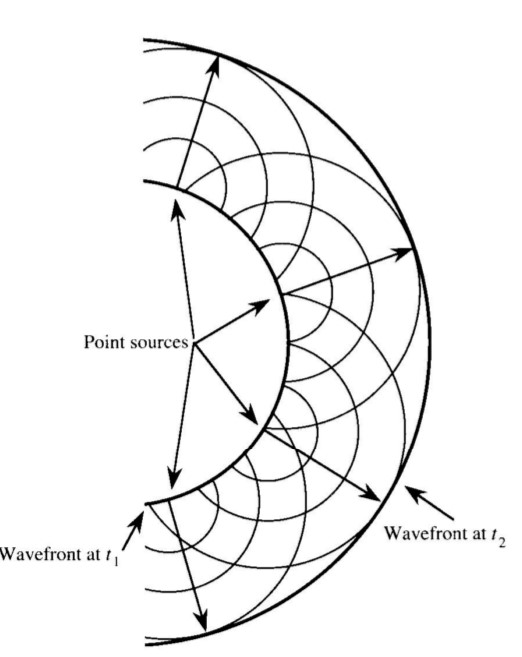
\includegraphics[height=0.5\textheight]{Images/huygens.jpg}
    \end{figure}
\end{frame}

\begin{frame}{Young's Double-Slit Experiment}
    \begin{figure}[htbp]
        \centering
        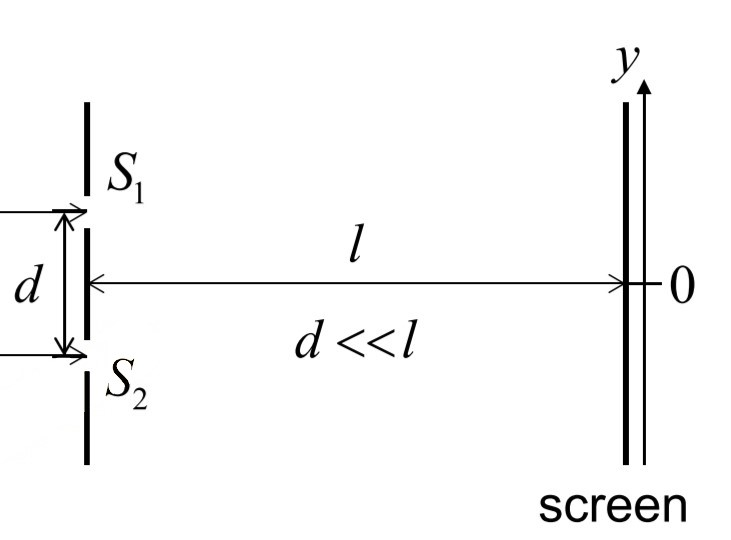
\includegraphics[height=0.5\textheight]{images/young.jpg}
        %\caption{}
        %\label{Fig:}
    \end{figure}

    If $d\ll l$, $\Delta \approx d\sin\theta \approx d \frac{y}{l}$.
    \begin{itemize}
        \item Constructive: $\Delta=m\lambda$
        \item Destructive: $\Delta= (2m+1)\lambda/2$
        \item $\abs{y_m} = m\lambda l/d$
    \end{itemize}
\end{frame}

\begin{frame}{Interference in Thin Films}
    \begin{beamerboxesrounded}[shadow=true]{Fresnel Equations}
        \begin{equation}
            E_{reflected} = \frac{n_1\cos\theta_{incident}-n_2\cos\theta_{reflected}}{n_1\cos\theta_{incident}+n_2\cos\theta_{reflected}} E_{incident}
        \end{equation}
        Sign changes $\Rightarrow$ phase change by $\pi$
    \end{beamerboxesrounded}
    \vspace{.5em}
    Other examples:
    \begin{itemize}
        \item Soap bubbles, oil specks
        \item Inclined thin films
        \item Coatings: non-reflective, reflective
        \item Newton rings (circular)
    \end{itemize}
\end{frame}

\begin{frame}{Diffraction}
    \begin{figure}[htbp]
        \centering
        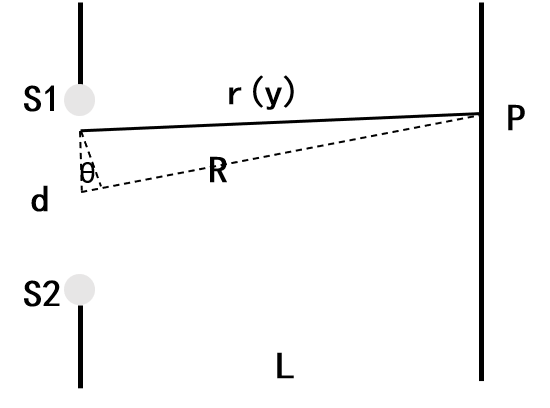
\includegraphics[scale=0.3]{images/diffraction.png}
    \end{figure} 
    
    Point wave on P:
    \begin{equation}
        \begin{split}
            \tilde{E}(r) &= \frac{E_A}{R}\exp(i(kr-\omega t)) \\
            r(y) &= R - y\sin\theta
        \end{split}
    \end{equation}

    Total wave:
    \begin{equation}
        \begin{split}
            \tilde{E}_P &= \frac{E_A}{R} \int_{-d/2}^{d/2} \exp(i(kR - \omega t)) \dd y \\ 
            &= \frac{E_A D}{R} \exp(i(kR-\omega t)) \frac{\sin\beta }{\beta} ,\ \beta = \frac{kD\sin\theta}{2}
        \end{split}
    \end{equation}

\end{frame}

\begin{frame}{Diffraction}
    Therefore, for single slit, the intensity is
    \begin{equation}
        \frac{I}{I_{max}} = (\frac{\sin\beta}{\beta})^2
    \end{equation}
    (half wave zone method)

    Other examples:
    \begin{itemize}
        \item Rectangular aperture: 
        \begin{equation}
            \frac{I}{I_{max}} = (\frac{\sin\alpha}{\alpha})^2(\frac{\sin\beta}{\beta})^2
        \end{equation}
        \item Circular aperture (first Bessel function): 
        \begin{equation}
            \frac{I(\theta)}{I_{max}} = (\frac{2J_1(ka\sin\theta)}{ka\sin\theta})^2
        \end{equation}
    \end{itemize}
\end{frame}

%----------------------------------------------------------------------------------------
%	 Section 2
%----------------------------------------------------------------------------------------

\section{Exercise}

\subsection{Ampere's Law}

\begin{frame}{Problem 1}
    There is a constant current density \textit{\textbf{j}} flowing between two cylindrical surfaces. Please find out the distribution of magnetic field inside the small cylindrical surface.
    \vfill
    \begin{figure}[H]
        \centering
        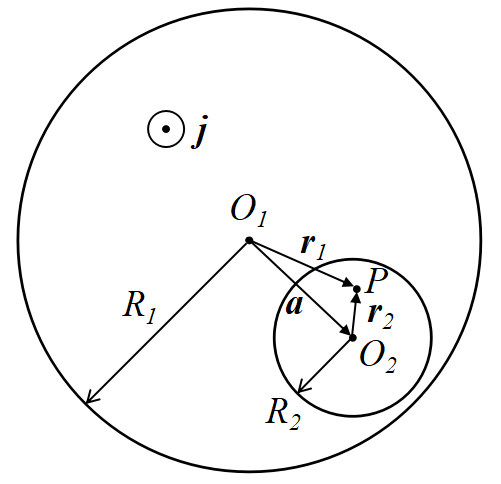
\includegraphics[width=0.30\textwidth]{images/008.png}
    \end{figure}
\end{frame}

\begin{frame}{Hw7.6}
Is Ampere’s law consistent with the general rule that you know from calculus that divergence of curl is always zero? Show that Ampere’s law cannot be valid, in general, outside magnetostatics.

Hint. The continuity equation.

\end{frame}

\subsection{Electromagnetic Induction}

\begin{frame}{Problem 2}
    Two identical capacitors with capacitance $C$ (zero charge) connected to each metal bar respectively (negligible resistance). Now put the system in an inward uniform magnetic field with magnitude $B$. Then give the metal bar an initial speed $v_{0}$ pointing to the right, please find out the final speeds of two metal bars respectively. 

\begin{figure}[H]
 \centering
 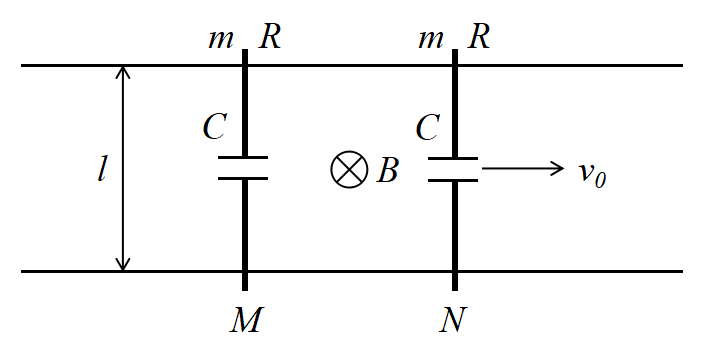
\includegraphics[width=0.65\textwidth]{images/010.png}
\end{figure}
    
\end{frame}


\begin{frame}{Problem 3}

    The rate of change of the magnetic field is $\mathrm{d}B/\mathrm{d}t=k>0$. 
    \begin{itemize}
        \item[(a)] If we put a metal bar $AB$ with length $R$ to satisfy that $OA=OB=AB=R$, then what will be the induced emf $\varepsilon_{AB}$? 
        \item[(b)] If we extend the metal bar to point $C$ outside the circular region such that $AB=BC=R$, what will be the induced emf $\varepsilon_{AC}$?
    \end{itemize}
    
\begin{figure}[H]
 \centering
 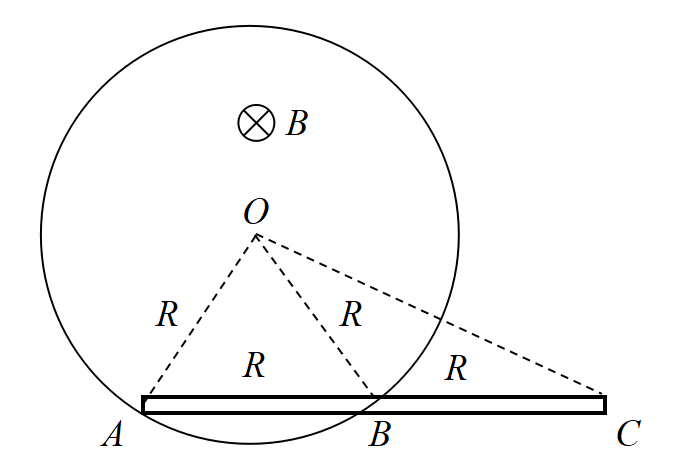
\includegraphics[width=0.5\textwidth]{images/013.png}
\end{figure}
    
\end{frame}


\begin{frame}{Hw9.5}
    \begin{figure}[htbp]
        \centering
        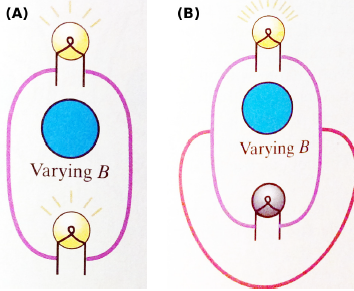
\includegraphics[scale=0.8]{images/hw9_5.png}
    \end{figure}
\end{frame}

\begin{frame}{Problem 4}
    A particle ($m$,$+q$) is given an initial speed $v_{0}$ pointing towards the center of a circular region. The radius of the circular region is $R$, and there is an inward uniform but varying magnetic field in this region ($\mathrm{d}B/\mathrm{d}t=k>0$). The particle touches the boundary of the circular region in a tangent trajectory after time t. When it touches the boundary of the circular region, the deflection angle is found to be $\theta$. Please find out the initial speed $v_{0}$.
 
\begin{figure}[H]
 \centering
 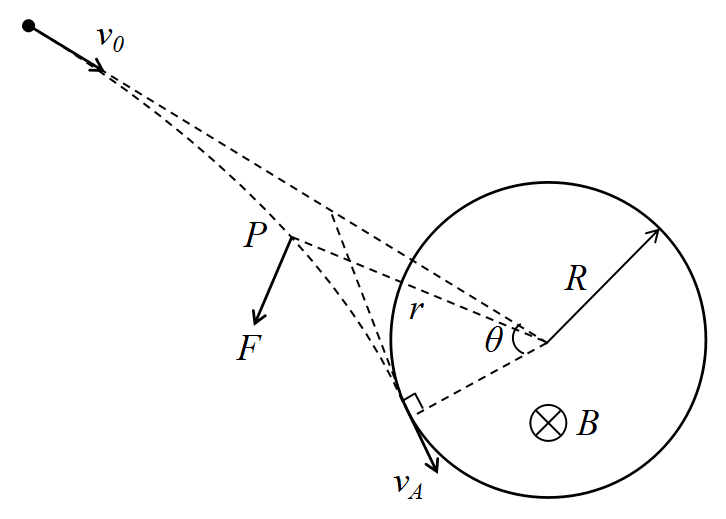
\includegraphics[width=0.5\textwidth]{images/015.png}
 \end{figure}
\end{frame}


\subsection{RLC \& AC Circuits}

\begin{frame}{Hw9.8}

The current travels in the same sense around each coil. One coil has self-inductance $L_1$, and the other coil has self-inductance $L_2$. The mutual inductance of the two coils is M. Show that if the two coils are connected in parallel, the equivalent inductance of the combination is $L = \frac{L_1L_2-M^2}{L_1+L+2-2M}$:

\end{frame}

\begin{frame}{Hw9.9}
    Sketch a qualitative graph of the reading of voltmeter $V_2$ as a function of time.

    \begin{figure}[htbp]
        \centering
        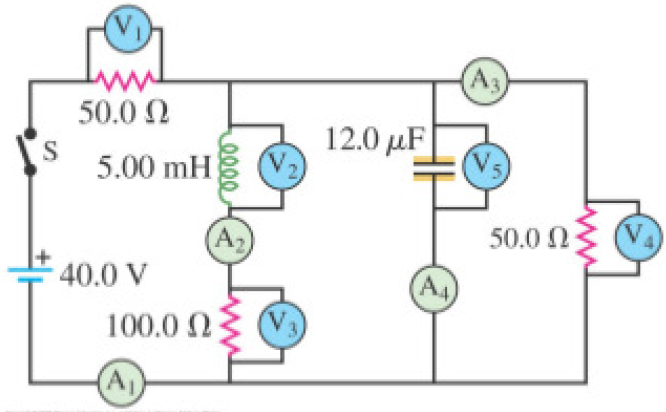
\includegraphics[scale=0.8]{images/hw9_9.png}
        %\caption{}
        %\label{Fig:}
    \end{figure}
\end{frame}


\subsection{Electromagnetic Waves}

\begin{frame}{Hw10.5}
    Rewrite the classical wave equation $\frac{\partial^{2} \xi(x, t)}{\partial x^{2}}-\frac{1}{v^{2}} \frac{\partial^{2} \xi(x, t)}{\partial t^{2}}=0$ using new variables $\alpha=x+v t$, $\beta=x-v t$ and show that any solution of this equation may be expressed as a sum of a wave traveling to the left and a wave traveling to the right, i.e. $\xi(x, t)=\xi_{1}(x+v t)+\xi_{2}(x-v t)$.
\end{frame}

\begin{frame}{Hw10.7}
    \small
    Electromagnetic waves propagate much differently in conductors than they do in dielectrics or in vacuum. If the resistivity of the conductor is sufficiently low (that is, if it is a sufficiently good conductor), the oscillating electric field of the wave gives rise to an oscillating conduction current that is much larger than the displacement current. In this case, the wave equation for an electric field $\mathbf{E}(x, t)=\left(0, E_{y}(x, t), 0\right)$ propagating in the $+x$ direction within a conductor is
$$
\frac{\partial^{2} E_{y}(x, t)}{\partial x^{2}}=\frac{\mu}{\rho} \frac{\partial E_{y}(x, t)}{\partial t}
$$
where $\mu$ is the permeability of the conductor and $\rho$ is its resistivity.
\end{frame}

\subsection{Optics}

\begin{frame}{Problem 5}

    \small
    There is a device called Lloyd mirror shown in figure. The source $S$ is placed at $s=2mm$ above the mirror. The distance between the source and the screen is $l=1.5m$ and the length of the mirror is $L=40cm$. The mirror is placed exactly at the middle between the source and the screen. It can generate an interference pattern on the screen. Please find out for the light with wavelength $\lambda=500nm$ the interval between bright fringes. Will fringes appear on the entire screen? If not, what is the range on the screen that fringes will appear?

\begin{figure}[htbp]
    \centering
    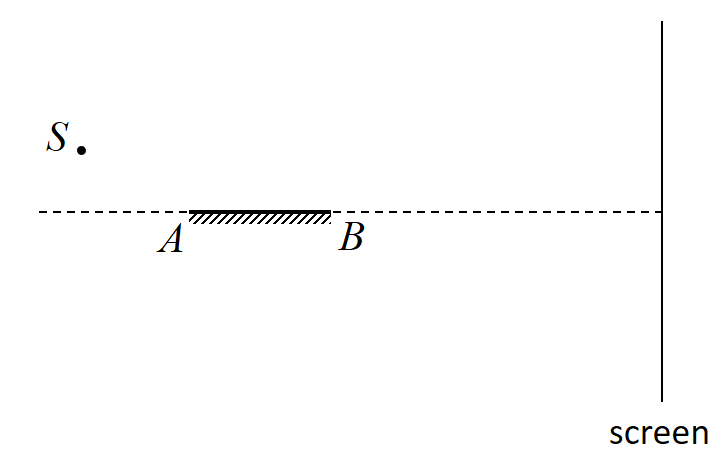
\includegraphics[scale=0.6]{images/005.png}
\end{figure}

\end{frame}

%----------------------------------------------------------------------------------------
%	 CLOSING/SUPPLEMENTARY SLIDES
%----------------------------------------------------------------------------------------
\section*{Appendix}

\begin{frame}
    \begin{center}
        \LARGE\bf LALALA
    \end{center}

\end{frame}

%----------------------------------------------------------------------------------------

\begin{frame}{\bf References}
    \nocite{*} % Display all references regardless of if they were cited
    \bibliography{example.bib}
    \bibliographystyle{plain}
\end{frame}

\end{document}

